\section{Deployment}
This section describes deployment architectures that are possible with Spring XD.
Note that this is not an exhaustive list of all 
deployment types, see section~\ref{sec:Use Cases} for descriptions of real 
world deployments.

\subsection{Streams and Batch Jobs}

XD provides the building blocks to create an event based system as well as
execute batch jobs on existing data.  

\subsubsection {Streams}
A basic stream defines the ingestion of event driven data from 
a source (see~\ref{sec:Source}) to a sink  (see~\ref{sec:Sink}) that passes 
through any number of processors (see~\ref{sec:Source}).  Spring XD streams can
also integrate with other event based solutions such as Apache Spark Streaming.

For example, the following stream definition can be used to ingest 
MQTT\cite{mqtt} data sent by a number of sensors directly into HDFS:

\verb;stream create ingest --definition "mqtt | hdfs";

In a more elaborate setting, an application can collect data from
different sources, and Spring XD can provide the means to merge them
in a single sink. The streams \texttt{in-mqtt} and \texttt{in-http}
collect data from sensors via MQTT and HTTP, respectively, and
contribute to a single queue \texttt{hdfs-in}. The merged result
is saved into HDFS.

\verb;stream create in-mqtt --definition ;\\*
\verb;  "mqtt > queue:hdfs-in";

\verb;stream create in-http --definition  ;\\*
\verb;  "http > queue:hdfs-in";

\verb;stream create ingest --definition  ;\\*
\verb;  "queue:hdfs-in > hdfs";

Processor modules in a stream offer the ability to transform, filter,
enrich data as it moves from one module to another.  In the example below
the stream will accept data from a http source and filter out any message
that does not have the word \emph{ocean} and then transform the message 
to all caps:

\verb;stream create oceanStream --definition "http |;\\*
\verb; filter --expression=payload.contains('ocean') |;\\*
\verb; transform --expression=payload.toUpperCase() |;\\*
\verb; hdfs";

In cases that a stream should be deactivated but the definition of the stream
should be maintained, the stream can be \emph{undeployed} as shown below:

\verb;stream undeploy  oceanStream ;

If the stream is no longer needed it can be \emph{destroyed} as shown below:

\verb;stream destroy  oceanStream ;

\subsubsection {Batch Jobs}

Spring XD allows users to create batch workflow solutions that span traditional
use-cases such as moving data between flat files and relational databases as 
well as Hadoop use-cases where analysis logic is broken up into several steps 
that run on a Hadoop cluster. Spring XD can deploy and launch a Spark application 
as a batch job.  The example below shows an example of creating a
job definition in XD.

\verb;job create sensorProcess;\\*
\verb;  --definition "sensors";

(This example already assumes an existing module job named \emph{sensors} that
implements the processing logic).

An important feature of the Spring XD is the regular
execution of jobs, as well as the ability to replay older datasets, for
instance reconstructing the \emph{data views} in case of loss or error.
The following mechanisms are available:

\begin{itemize*}
\item \emph{manual} job launch through its shell user interface or 
administrative UI;
\item \emph{stream-controlled} where the jobs are launched by a stream of 
\emph{trigger} messages;
\item \emph{scheduled} job launch according to a \texttt{cron} expression;
\end{itemize*}

For example, a job can be launched manually as follows:

\verb;job launch sensor-process;

Or, more typically, it can be launched on a schedule:

\verb;stream create --name launchSensorProcess;\\*
\verb;  --definition "trigger --cron=`0/5 * * * * *';\\* 
\verb;  > queue:job:myCronJob" --deploy;

\subsubsection {Blending Streams and Jobs}

Spring XD offers the ability for streams and jobs to work together in that
a stream can launch a job or a stream can received notifications from a job
as it is executing.  In the example below an http source will pass the http
payload to the "myHttpJob, thus launching the job:

\verb;stream create --name jobStream --definition ;\\*
\verb; "http > queue:job:myHttpJob" --deploy;

In the example below a stream will receive all events from a job and write 
the data to the log:

\verb;job create --name myHttpJob --definition;\\* 
\verb; "httpJob" --deploy;\\*
\verb;stream create --name aggregatedEvents --definition;\\*
\verb; "tap:job:myHttpJob >log" --deploy;\\*
\verb;job launch myHttpJob;

\subsection {Reactive applications}

The last few years have seen a significant change in application requirements:
data volumes of terabyte order, response times within tens of milliseconds, stricter
availability requirements. These new challenges require a new approach to application
development, subsumed under the concepts of \emph{reactive applications} and \emph{reactive
programming}. In what follows next, we will describe how these concepts are
illustrated by Spring XD, both from a runtime platform, as well as from a development perspective.

\subsubsection {Spring XD as a platform for \\ reactive applications}

Reactive applications, as described by the Reactive \linebreak Manifesto
\cite{reactive} are \emph{responsive}, \emph{resilient}, \emph{elastic}
and \emph{message driven}. Spring XD, as a platform, provides the means for creating and
running reactive applications.

\emph{Responsiveness} represents a system's ability to respond in a timely manner, if
at all, possible. In the case of Spring XD, its stream processing model is designed
for building fast, low-latency data pipelines.

\emph{Resilience} represents a system's ability to remain responsive in the face of
failure. In Spring XD, this is provided out of the box by features such as automatic
module redeployment if the host container has crashed, or the ability to elect a new
admin node in case the existing one fails. On a more granular level, automatic retry
and dead-letter queue support for RabbitMQ and Redis allows tracking and recovery
from failed computations. The use of messaging middleware ensures redelivery of data
when a module recovers.

\emph{Elasticity} represents a system's ability to remain responsive under varying
workload. In Spring XD, this is provided by features such as the ability to scale up
the processing power by deploying multiple instances of a module or job in a stream.

\emph{Message-driven} represents a system's reliance on \linebreak
asynchronous message passing between components. This is a core
feature of Spring XD, implemented by its message bus (see~\ref{subsec:MessageBus}).

This is how Spring XD as a platform allows applications to meet the criteria for being
considered \emph{reactive}. In conjunction with that, it provides the ability of using
a development model that is better suited for reactive applications, through its support
for \emph{reactive programming} and \emph{observable streams}.

\subsubsection {Reactive programming and functional \\ in Spring XD}

\emph{Reactive programming} is a programming paradigm centered around asynchronous
stream processing. The central notion is that incoming data can be processed in an
ordered, asynchronous and event-driven manner, using functional operators to describe
transformations that apply to an entire stream of incoming data. The operators can
vary from individual item transformations, to grouping and aggregation over given
time windows, and can be composed into complex data processing pipelines that produce
outbound streams of data.

ReactiveX~\cite{reactivex} is one of the most common set of APIs, centered around
the \texttt{Observable} abstraction that extends the observer pattern to streams,
together with a rich set of operators for composing and transforming sequences, and
RxJava~\cite{rxjava} is the Java implementation of the ReactiveX API. 

Spring XD provides support for reactive programming \linebreak
through a special type of processors that transform asynchronous
streams of data. The API for RxJava is supported. An example of an RxJava 
processor is shown in figure \ref{fig:rxjava}.
Spring XD has the responsibility of transforming the 
flow of discrete messages arriving on a processor's input channel into an
RxJava \texttt{Observable}, as well as transforming the \texttt{Observable} 
returned by the processor module into a flow of discrete messages sent on 
the output channel. Inside the processor, RxJava operators are applied for 
performing transformations on the data stream.

\begin{figure}[ht]
\centering
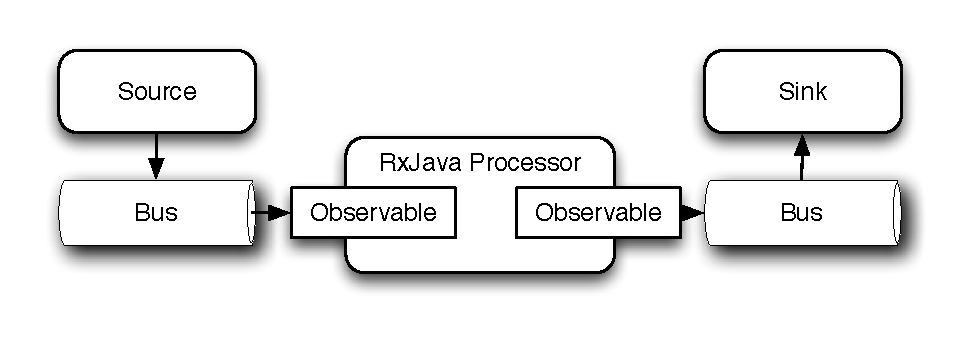
\epsfig{file=rxjava.eps, height=2in, width=3in}
\caption{Reactive module using RxJava}
\label{fig:rxjava}
\end{figure}

